\subsection{Dependency Probing (RQ4)}
\label{sec:rq4}

\begin{figure}[t]
 	\centering
 	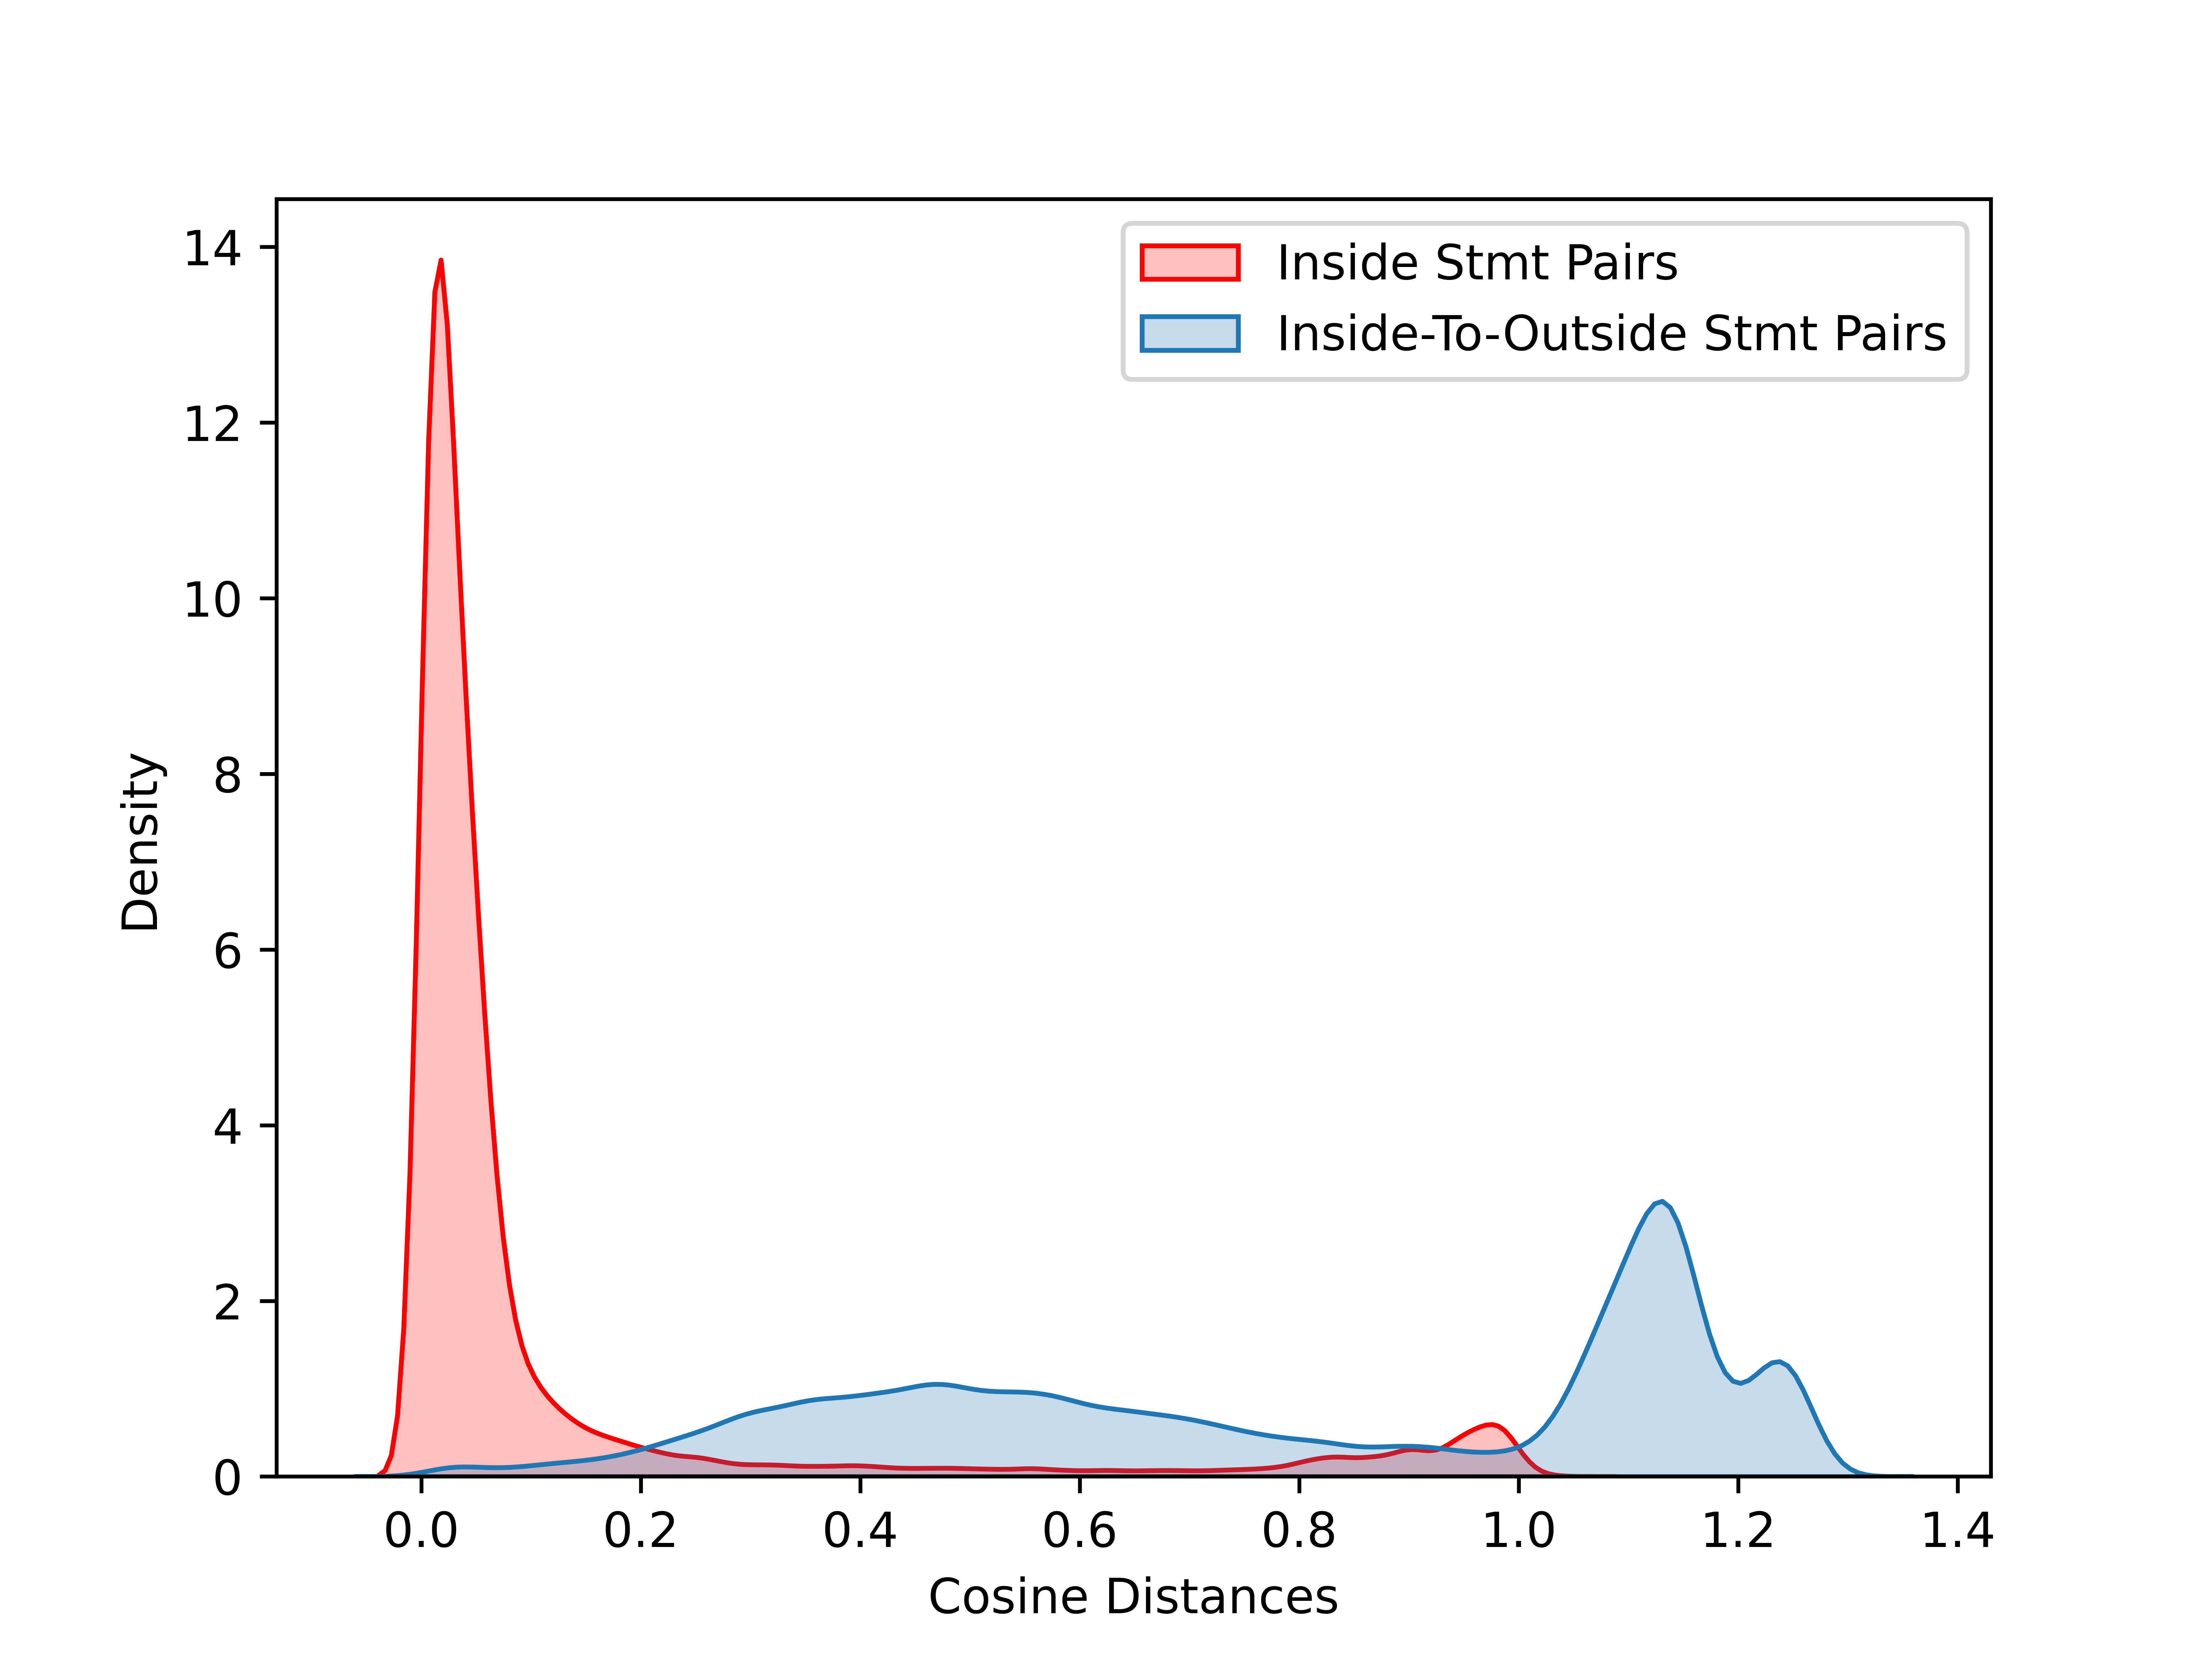
\includegraphics[width=2.2in]{rq4-density.png}
        \vspace{-12pt}
 	\caption{The Distribution of Cosine Distances}
 	\label{fig:rq4-density}	
\end{figure}

The confidence interval of the mean of cosine distances for the inside
statement group is 0.1262 to 0.1268 with 95\% confidence, and the
confidence interval for the inside-to-outside statement group is
0.7987 to 0.8001 with 95\% confidence. As seen in
Figure~\ref{fig:rq4-density}, the distribution of the cosine distances
for all the inside-to-outside statement pairs is largely to the right
of the distribution for all the inside statement pairs. That is,
{\tool} tends to {\em encode statements in a way that the statements
  in the same \code{try-catch} block are closer to each other in the
  embedding space}, leading to better grouping.


